% Main figure 1 -- workflow of the RI-RS G0W0 space-time algorithm.
%
% Same idea as Figure 1 of Wilhelm, Seewald, Golze, JCTC 17, 1662 (2021):
% one box per step with the working equation inside (title left-aligned,
% equations centred).  Sized for ONE column
% of the REVTeX two-column layout (drawn at natural size, ~8.4 cm wide, so
% that \includegraphics[width=\linewidth] does not rescale the fonts).
%
% The sparse grid steps are blue, the two dense steps (W and the QP step)
% orange.  The label in the top-right corner of each box is the FORMAL
% scaling of that step for large systems, i.e. once the AO cutoff r_AO, the
% truncated Coulomb metric (r_c) and the cutoff r_W make Phi, Z and the grid
% representations of G and W sparse: the grid steps are then O(N), the dense
% steps in the auxiliary / molecular-orbital basis O(N^3).  (The measured
% exponents are in Fig. 4c.)  The input box has no scaling label.
%
% Build:   cd script && pdflatex -output-directory=../fig fig1_workflow.tex
%
\documentclass[border=2pt]{standalone}\usepackage{amsmath,amssymb}\usepackage{bm}
\usepackage{upgreek}
\usepackage{tikz}
\usetikzlibrary{positioning,arrows.meta,calc}
\usepackage[T1]{fontenc}
\usepackage{newtxtext,newtxmath}   % Times-like, matches the REVTeX text font

% colours: blue = sparse grid step, orange = dense step
\definecolor{sparse}{HTML}{3C5488}   % = RI-RS colour of all plots
\definecolor{dense}{HTML}{E18727}
\definecolor{ink}{HTML}{111111}
\definecolor{inp}{HTML}{7f7f7f}
\definecolor{spgreen}{HTML}{0B6E4F}   % sparse matrices are written in this colour
\newcommand{\spm}[1]{{\color{spgreen}#1}}

\tikzset{
  step/.style={draw=#1, line width=0.8pt, fill=#1!7, rounded corners=2.5pt,
               text width=7.75cm, align=left, inner sep=4pt, text=ink,
               font=\footnotesize},
  num/.style={circle, fill=#1, text=white, font=\bfseries\scriptsize,
              inner sep=1pt, minimum size=11pt},
  scal/.style={font=\footnotesize, text=#1, anchor=north east, inner sep=3pt},
  arr/.style={-{Latex[length=1.8mm]}, line width=0.8pt, draw=ink!70},
}

\begin{document}
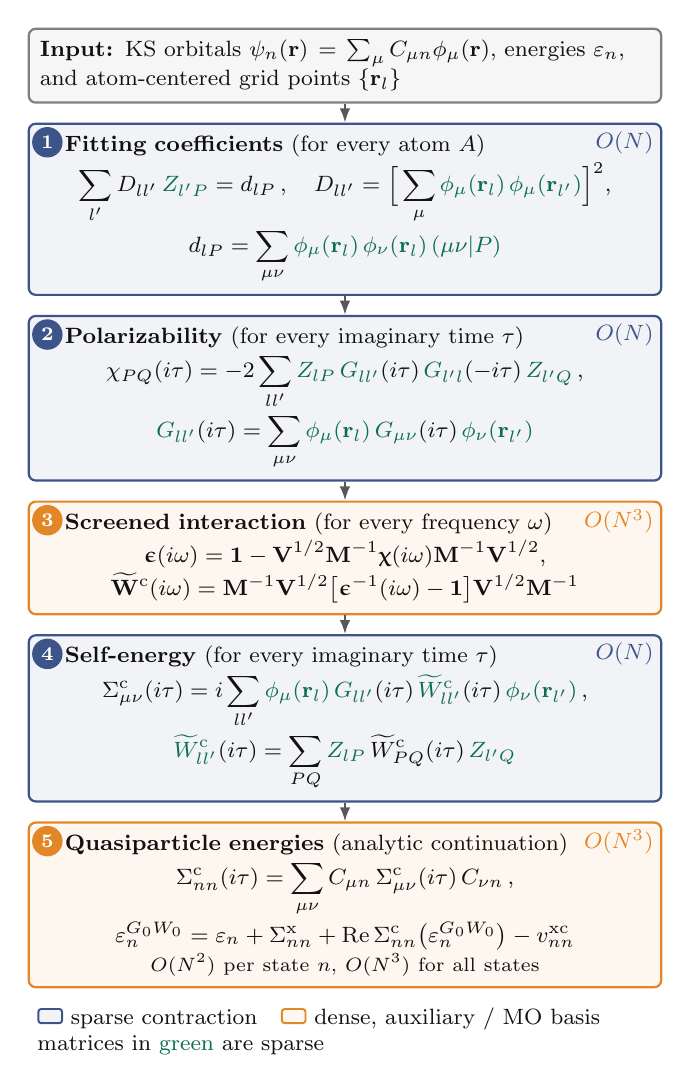
\begin{tikzpicture}[node distance=2.4mm]

% ---- input -----------------------------------------------------------------
\node[step=inp] (in) {%
  \textbf{Input:} KS orbitals $\psi_n(\mathbf r)=\sum_\mu C_{\mu n}\phi_\mu(\mathbf r)$,
  energies $\varepsilon_n$, and atom-centered grid points $\{\mathbf r_l\}$\par};

% ---- 1: fitting coefficients ---------------------------------------------
\node[step=sparse, below=of in] (s1) {%
  \hspace{9pt}\textbf{Fitting coefficients} (for every atom $A$)\par\vspace{1pt}\centering
  $\displaystyle \sum_{l'} D_{ll'}\, \spm{Z_{l'P}} = d_{lP}\,,\quad
   D_{ll'}=\Big[\sum_\mu \spm{\phi_\mu(\mathbf r_l)}\,\spm{\phi_\mu(\mathbf r_{l'})}\Big]^2,$\par\vspace{1pt}
  $\displaystyle d_{lP}=\sum_{\mu\nu}\spm{\phi_\mu(\mathbf r_l)}\,\spm{\phi_\nu(\mathbf r_l)}\,\spm{(\mu\nu|P)}$\par};

% ---- 2: polarizability -----------------------------------------------------
\node[step=sparse, below=of s1] (s2) {%
  \hspace{9pt}\textbf{Polarizability} (for every imaginary time $\tau$)\par\vspace{1pt}\centering
  $\displaystyle \chi_{PQ}(i\tau) = -2\sum_{ll'} \spm{Z_{lP}}\,
     \spm{G_{ll'}}(i\tau)\,\spm{G_{l'l}}(-i\tau)\,\spm{Z_{l'Q}}\,,$\par\vspace{1pt}
  $\displaystyle \spm{G_{ll'}}(i\tau)=\sum_{\mu\nu}\spm{\phi_\mu(\mathbf r_l)}\,
     \spm{G_{\mu\nu}}(i\tau)\,\spm{\phi_\nu(\mathbf r_{l'})}$\par};

% ---- 3: screened interaction -----------------------------------------------
% includes the multiplication with M^-1 from both sides, so that box 4 uses
% the result directly (M^-1 W M^-1 is a dense O(N^3) step and belongs here)
\node[step=dense, below=of s2] (s3) {%
  \hspace{9pt}\textbf{Screened interaction} (for every frequency $\omega$)\par\vspace{1pt}\centering
  $\displaystyle \bm{\upepsilon}(i\omega) = \mathbf{1} - \mathbf{V}^{1/2}\mathbf{M}^{-1}\bm{\upchi}(i\omega)\mathbf{M}^{-1}\mathbf{V}^{1/2},$\par\vspace{1pt}
  $\displaystyle \widetilde{\mathbf{W}}^\text{c}(i\omega) = \mathbf{M}^{-1}\mathbf{V}^{1/2}\big[\bm{\upepsilon}^{-1}(i\omega)-\mathbf{1}\big]\mathbf{V}^{1/2}\mathbf{M}^{-1}$\par};

% ---- 4: self-energy ----------------------------------------------------------
\node[step=sparse, below=of s3] (s4) {%
  \hspace{9pt}\textbf{Self-energy} (for every imaginary time $\tau$)\par\vspace{1pt}\centering
  $\displaystyle \Sigma^\text{c}_{\mu\nu}(i\tau) = i\sum_{ll'}\spm{\phi_\mu(\mathbf r_l)}\,
     \spm{G_{ll'}}(i\tau)\,\spm{\widetilde W^\text{c}_{ll'}}(i\tau)\,\spm{\phi_\nu(\mathbf r_{l'})}\,,$\par\vspace{1pt}
  $\displaystyle \spm{\widetilde W^\text{c}_{ll'}}(i\tau) = \sum_{PQ} \spm{Z_{lP}}\,\widetilde W^\text{c}_{PQ}(i\tau)\,\spm{Z_{l'Q}}$\par};

% ---- 5: QP energies ----------------------------------------------------------
\node[step=dense, below=of s4] (s5) {%
  \hspace{9pt}\textbf{Quasiparticle energies} (analytic continuation)\par\vspace{1pt}\centering
  $\displaystyle \Sigma^\text{c}_{nn}(i\tau) = \sum_{\mu\nu} C_{\mu n}\,\Sigma^\text{c}_{\mu\nu}(i\tau)\,C_{\nu n}\,,$\par\vspace{1pt}
  $\displaystyle \varepsilon_n^{G_0W_0} = \varepsilon_n + \Sigma^\text{x}_{nn}
     + \text{Re}\,\Sigma^\text{c}_{nn}\big(\varepsilon_n^{G_0W_0}\big) - v^\text{xc}_{nn}$\par\vspace{1pt}
  {\scriptsize $O(N^2)$ per state $n$, $O(N^3)$ for all states}\par};

% ---- arrows ----------------------------------------------------------------
\foreach \a/\b in {in/s1, s1/s2, s2/s3, s3/s4, s4/s5}
  \draw[arr] (\a.south) -- (\b.north);

% ---- step numbers, in the top-left corner of each box ------------------------
\foreach \s/\c/\n in {s1/sparse/1, s2/sparse/2, s3/dense/3, s4/sparse/4, s5/dense/5}
  \node[num=\c] at ($(\s.north west)+(0.25,-0.25)$) {\n};

% ---- formal scaling, in the top-right corner of each box -------------------
\node[scal=sparse] at (s1.north east) {$O(N)$\par};
\node[scal=sparse] at (s2.north east) {$O(N)$\par};
\node[scal=dense]  at (s3.north east) {$O(N^3)$\par};
\node[scal=sparse] at (s4.north east) {$O(N)$\par};
\node[scal=dense]  at (s5.north east) {$O(N^3)$\par};

% ---- legend -----------------------------------------------------------------
\node[anchor=north west, font=\footnotesize, text=ink, align=left]
  at ($(s5.south west)+(0,-0.12)$) {%
  \tikz\fill[sparse!7, draw=sparse, line width=0.7pt, rounded corners=1pt] (0,0) rectangle (0.3,0.18);\
  sparse contraction\quad
  \tikz\fill[dense!7, draw=dense, line width=0.7pt, rounded corners=1pt] (0,0) rectangle (0.3,0.18);\
  dense, auxiliary / MO basis\\
  matrices in \spm{green} are sparse};

\end{tikzpicture}
\end{document}
